\section*{Problem 3: Velocity Kinematics} \label{Sec: Problem 3: Velocity Kinematics}


	In order to follow a contour at constant velocity, or at any prescribed velocity, we must
	know the relationship between the velocity of the tool and the joint velocities.
	In our case we can differentiate Equations (\ref{eq:positionX}) and (\ref{eq:positionY}) to obtain equations describing
	the velocity in the $x$ and $y$ direction. These equations will enable us to derive the \textbf{Jacobian} matrix of the manipulator,
	which is a fundamental object to determine for any manipulator.\\
	In Chapter 5 we present a systematic procedure for deriving the Jacobian for any manipulator in the so-called cross-product form.

	We can look at properties of the Jacobian to determine in which case the manipulator is said to be in a singular configuration,
	such as shown in Figure 1.28 for $\theta_2 = 0$:

	\begin{figure}[H]
		\centering
		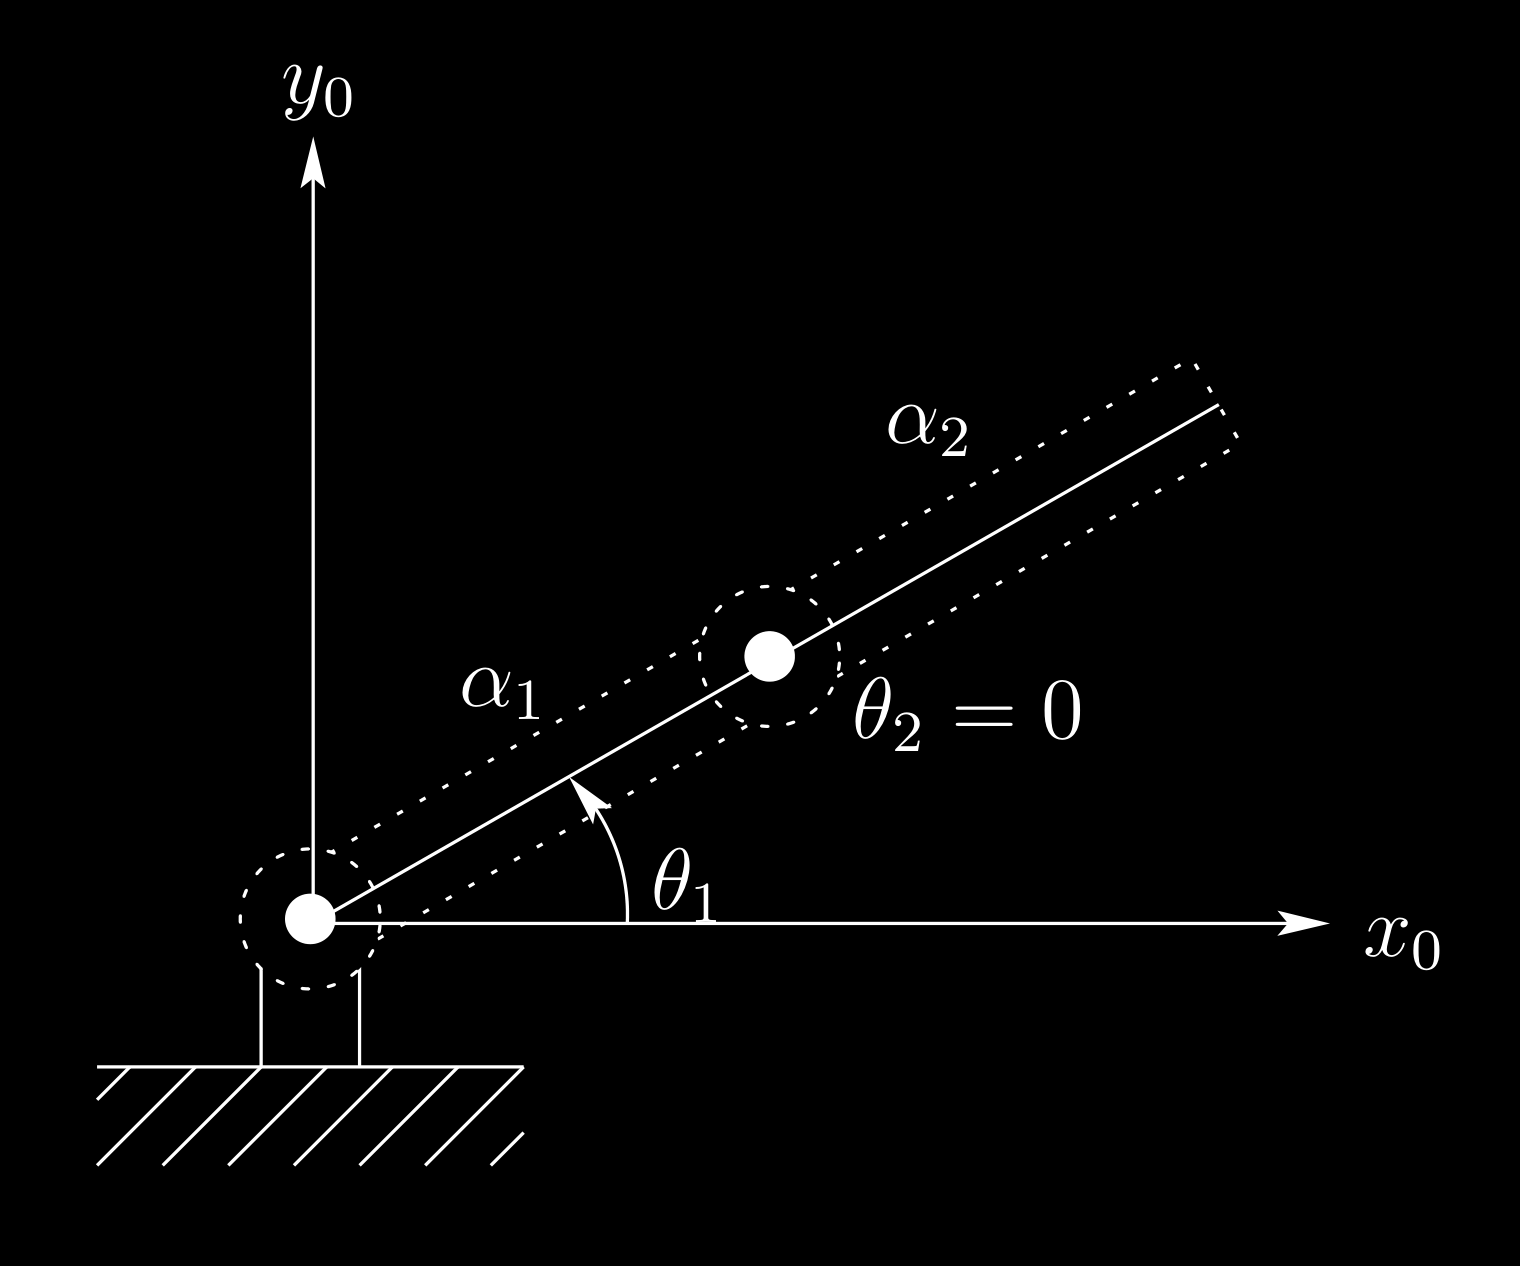
\includegraphics[width=0.9\textwidth]{img/Figure1_28.png}
		\caption{A singular configuration.}
		\label{fig:Figure1_28}
	\end{figure}

	The determination of such singular configurations is important for several reasons.
	At singular configurations there are infinitesimal motions that are unachievable; that is, the manipulator end-effector cannot move in certain directions.
	In the above cases the end effector cannot move in the direction parallel to $x_{2}$, from a singular configuration.
	Singular configurations are also related to the non-uniqueness of solutions of the inverse kinematics.
	For example, for a given end-effector position, there are in general two possible solutions to the inverse kinematics.
	Note that the singular configuration separates these two solutions in the sense that the manipulator cannot go from one
	configuration to the other without passing through the singularity.
	For many applications it is important to plan manipulator motions in such a way that singular configurations are avoided.
